\documentclass[journal]{IEEEtran}
\usepackage{cite}
\usepackage{amsmath,amssymb,amsfonts}
\usepackage{algorithmic}
\usepackage{graphicx}
\usepackage{textcomp}
\usepackage{xcolor}
\usepackage{tikz}
\usetikzlibrary{shapes.geometric, arrows, positioning, fit, calc}
\usepackage{booktabs}
\usepackage{multirow}
\usepackage{hyperref}

\begin{document}

\title{PRED: A Projection-Based Reference Defense against Stealthy Fairness Poisoning in Federated Learning}

\author{
\IEEEauthorblockN{Anonymous Authors}
}

\maketitle

\begin{abstract}
Federated Learning (FL) allows distributed clients to collaboratively train a global model without sharing raw data. However, FL is highly vulnerable to poisoning attacks, where malicious clients manipulate the global model. Recently, fairness poisoning attacks have emerged, specifically designed to degrade the model's fairness (e.g., Demographic Parity, Equal Opportunity) while preserving its overall predictive accuracy, making them incredibly difficult to detect using standard robust aggregation techniques. In highly non-IID data environments, these attacks easily blend in with the natural statistical variance of honest clients. In this paper, we propose PRED (Projection-based Reference Defense), a novel, dual-phase defense mechanism specifically designed to thwart stealthy fairness poisoning attacks. PRED leverages a tiny, server-side reference dataset to construct an importance-weighted fairness-gradient projection, allowing the server to isolate the precise direction of fairness violation. We introduce a per-round, memoryless exclusion protocol that identifies attackers using Median Absolute Deviation (MAD) on projection scores, preventing the permanent exclusion of honest minority clients. Furthermore, we demonstrate a critical finding: at extremely low attack ranks where detection is highly successful, excluding clients actually harms global fairness due to non-IID data starvation. Consequently, PRED integrates an unconditional, post-hoc fairness repair step that synergizes with detection, neutralizing stealthy attacks that evade the primary filter while preserving data volume. Extensive empirical evaluations across Adult Income, Bank Marketing, and ACSIncome datasets demonstrate that PRED consistently preserves state-of-the-art fairness ($\Delta$DP $< 0.12$) under advanced Low-Rank (LoRA) fairness attacks, outperforming traditional Byzantine-robust methods (Krum, FLTrust) and contemporary fairness-aware defenses (GuardFed, DPG-FairFL).
\end{abstract}

\begin{IEEEkeywords}
Federated Learning, Fairness, Poisoning Attacks, Robust Aggregation, Byzantine Fault Tolerance.
\end{IEEEkeywords}

\section{Introduction}
Federated Learning (FL) \cite{mcmahan2017communication} has emerged as the premier paradigm for privacy-preserving machine learning. By decentralizing the training process, FL enables mobile devices, hospitals, and financial institutions to collaboratively optimize a shared global model while retaining their raw, sensitive data locally. Despite its privacy benefits, the distributed nature of FL introduces severe security vulnerabilities. Because the central server cannot inspect the raw data of the participating clients, the federation is fundamentally exposed to poisoning attacks, where malicious actors inject corrupted local model updates to compromise the global aggregate. 

While traditional poisoning attacks seek to degrade the global model's overall utility (untargeted poisoning) or force the model to misclassify specific inputs (backdoor attacks), a new, insidious threat vector has recently been identified: fairness poisoning \cite{lorafl2024}. In a fairness poisoning attack, the adversary specifically targets the demographic equity of the model. The objective is to maximize the disparity in predictive outcomes across sensitive attributes (such as race, gender, or age) while meticulously preserving the model's overall test accuracy. This creates a stealthy attack footprint. Standard Byzantine-robust aggregation methods, which typically filter updates based on geometric distances or gradient magnitudes, are blind to these attacks because the malicious updates do not degrade the primary objective function. The problem is exacerbated in highly non-IID (non-Independent and Identically Distributed) environments, where honest clients naturally exhibit highly divergent gradients. In such settings, an attacker can easily camouflage their fairness-degrading perturbation within the natural statistical variance of the honest federation.

Defending against fairness poisoning requires mechanisms that can explicitly measure the semantic intent of a local update. Existing reference-based defenses, such as FLTrust \cite{cao2021fltrust}, attempt to bootstrap trust using a clean server-side dataset, but they optimize for general utility rather than fairness. Recent fairness-specific defenses, such as GuardFed \cite{guardfed2024} and DPG-FairFL \cite{dpgfairfl2025}, attempt to audit updates for fairness violations. However, as our evaluations demonstrate, these methods frequently collapse in non-IID settings. When honest clients possess heavily skewed local datasets (e.g., an extreme class imbalance), their legitimate updates appear highly biased. Existing defenses routinely falsely flag these honest updates as malicious, leading to catastrophic utility degradation or complete model collapse.

To address this critical vulnerability, we propose PRED (Projection-based Reference Defense), a robust, dual-phase defense mechanism tailored for non-IID federated environments. PRED utilizes a small server-side reference dataset to construct an explicit geometric representation of the fairness objective. By projecting client updates onto an importance-weighted reference gradient, PRED mathematically isolates the precise direction of fairness violation, stripping away the noise of non-IID objective gradients. We utilize a memoryless, per-round exclusion scoring mechanism based on Median Absolute Deviation (MAD), intentionally discarding historical suspicion metrics to prevent the permanent disenfranchisement of honest clients with skewed data.

Crucially, through extensive ablation studies, we uncover a counterintuitive property of FL defenses: accurate detection can actively harm fairness. We demonstrate that explicitly excluding clients—even when successfully removing the attacker—starves the global model of valuable data. In severely non-IID environments, this data starvation exacerbates the natural bias of the remaining honest clients, resulting in worse global fairness than if the attacker had been ignored. To counter this, PRED incorporates an unconditional, post-hoc fairness repair step. We show that the true strength of PRED lies in the synergy between its components: the detection module filters out the most aggressive attacks, while the repair module cleanly neutralizes the stealthy perturbations that evade detection, without dropping critical honest data.

The primary contributions of this paper are as follows:
\begin{enumerate}
    \item We introduce the Importance-Weighted Reference Projection, a novel geometric scoring mechanism that explicitly corrects for server-side class imbalances, effectively eliminating false positive exclusions in highly non-IID federated settings.
    \item We design PRED, a dual-phase defense that combines per-round memoryless exclusion with unconditional fairness repair, providing state-of-the-art resilience against stealthy Low-Rank (LoRA) fairness attacks.
    \item We conduct a rigorous, cross-dataset empirical evaluation against leading baselines (Krum, FLTrust, GuardFed, DPG-FairFL), demonstrating PRED's superiority in preserving both Demographic Parity and Equal Opportunity without sacrificing test accuracy.
    \item We present a comprehensive ablation analysis revealing that, at high detection rates, data starvation caused by client exclusion is more detrimental to fairness than the attack itself, fundamentally shifting the paradigm of robust aggregation from ``exclude'' to ``repair.''
\end{enumerate}

\section{Related Work}
\subsection{Traditional Byzantine-Robust Aggregation}
The vulnerability of FL to Byzantine failures and malicious poisoning has driven the development of numerous robust aggregation algorithms. Krum \cite{blanchard2017machine} operates by selecting a single client update that is geometrically closest to its peers, effectively discarding outliers. While Krum provides theoretical guarantees against minority Byzantine attackers, it fundamentally struggles in non-IID environments where honest client updates naturally form disparate clusters, causing Krum to arbitrarily favor one local distribution over others.

\subsection{Reference-Based Defenses}
To anchor the global model against extreme non-IID variance, reference-based defenses utilize a small, clean dataset on the server. FLTrust \cite{cao2021fltrust} computes a pristine gradient on this server root dataset and scores client updates based on their cosine similarity to this root gradient. Updates that align with the root gradient are assigned higher trust scores, and the global aggregation is performed as a weighted average. However, because the root gradient is computed using standard cross-entropy loss, FLTrust is entirely focused on general utility. It is fundamentally blind to orthogonal perturbations designed to degrade fairness, making it ineffective against targeted fairness poisoning.

\subsection{Fairness Poisoning Attacks}
Fairness poisoning is a relatively new subfield of adversarial machine learning. The LoRA-FL attack \cite{lorafl2024} represents the state-of-the-art in stealthy fairness degradation. Rather than manipulating the entire gradient vector, the LoRA-FL attacker projects their fairness-violating objective into a low-rank subspace (via low-rank matrix factorization). By constraining the attack to this subspace, the perturbation minimizes its footprint on the model's primary task loss. This allows the attacker to massively inflate metrics like the Demographic Parity gap while easily bypassing magnitude-clipping and distance-based defenses.

\subsection{Fairness-Aware FL Defenses}
Recent works have attempted to explicitly audit FL updates for fairness. GuardFed \cite{guardfed2024} attempts to detect attackers by evaluating the fairness of each client's update on a server-side validation set. However, GuardFed relies on strict, threshold-based rejections. As we demonstrate in this paper, GuardFed collapses in non-IID settings because honest clients with extreme local class imbalances naturally produce updates that appear ``unfair'' in isolation, leading to false rejection and model starvation. Similarly, DPG-FairFL \cite{dpgfairfl2025} attempts to use Dual-Phase GANs to synthesize balanced reference data for auditing. Unfortunately, GANs trained on tiny reference sets (e.g., 250 samples) are highly prone to mode collapse, particularly on tabular data, rendering the generated reference set useless for distinguishing subtle, low-rank fairness attacks from honest variance.

\section{Preliminaries and Threat Model}
\subsection{Federated Learning Formulation}
We consider a standard horizontal Federated Learning setting comprising a central server and a set of $N$ clients, indexed by $i \in \{1, \dots, N\}$. The goal of the federation is to collaboratively train a global machine learning model parameterized by weights $w \in \mathbb{R}^d$ to minimize a global objective function $F(w)$. 

At each communication round $t$, the server broadcasts the current global model weights $w_t$ to the clients. Each client $i$ performs local training on their private dataset $D_i$ to minimize their local empirical risk $F_i(w)$. Let the resulting local model weights be $w_t^i$. The client then computes their local update (or pseudo-gradient) as:
\begin{equation}
\Delta w_t^i = w_t^i - w_t
\end{equation}
This equation simply defines the vector difference between the locally optimized model and the global model broadcasted at the start of the round. The update $\Delta w_t^i$ encapsulates the knowledge learned by client $i$ during the current round. This specific formulation, transmitting updates rather than absolute weights, is chosen because it allows the server to explicitly analyze the magnitude and direction of the client's proposed changes, which is mathematically necessary for both Byzantine-robust filtering (e.g., Krum, FLTrust) and our projection-based defense.

The clients transmit their updates $\Delta w_t^i$ to the central server. The server aggregates these updates using a function $\text{Agg}(\cdot)$ to produce the new global model:
\begin{equation}
w_{t+1} = w_t + \text{Agg}\left(\{\Delta w_t^1, \dots, \Delta w_t^N\}\right)
\end{equation}
Here, $w_{t+1}$ represents the updated global model for the next round. The aggregation function $\text{Agg}$ takes the set of all submitted client updates and combines them into a single, global update step. The standard approach is Federated Averaging (FedAvg) \cite{mcmahan2017communication}, where $\text{Agg}$ is a simple weighted arithmetic mean based on dataset sizes. This formulation is the foundational mechanism of FL, chosen because it allows distributed optimization to converge towards the global optimum without requiring any client to transmit their raw, sensitive data $D_i$ to the server.

\subsection{Fairness Metrics}
We focus on binary classification tasks where the input data includes a sensitive attribute $S \in \{0, 1\}$ (e.g., gender or race), a target label $Y \in \{0, 1\}$, and a prediction $\hat{Y} \in \{0, 1\}$. To quantify the fairness of the global model, we utilize two standard metrics: Demographic Parity (DP) and Equal Opportunity (EO).

The Demographic Parity gap ($\Delta$DP) measures the difference in positive prediction rates between the two sensitive groups, regardless of the true label. It is defined as:
\begin{equation}
\Delta\text{DP} = \left| P(\hat{Y}=1 \mid S=1) - P(\hat{Y}=1 \mid S=0) \right|
\end{equation}
In this equation, $P(\hat{Y}=1 \mid S=1)$ represents the probability that the model predicts a positive outcome for the privileged group, while $P(\hat{Y}=1 \mid S=0)$ represents the probability for the unprivileged group. The absolute difference between these two rates is the $\Delta$DP. This metric was chosen because it explicitly captures disparate impact; a perfectly fair model under DP will grant the positive outcome at exactly the same rate to both groups, yielding a $\Delta$DP of zero. Attackers often target DP because violating it causes direct, measurable harm to specific demographics.

The Equal Opportunity gap ($\Delta$EO) measures the disparity in the model's ability to correctly identify positive instances across the sensitive groups. It requires that the True Positive Rate (TPR) and False Positive Rate (FPR) be equal across groups. It is defined as:
\begin{equation}
\Delta\text{EO} = \max\left( |\text{TPR}_{S=1} - \text{TPR}_{S=0}|, |\text{FPR}_{S=1} - \text{FPR}_{S=0}| \right)
\end{equation}
Here, $\text{TPR}_{S=s} = P(\hat{Y}=1 \mid Y=1, S=s)$ and $\text{FPR}_{S=s} = P(\hat{Y}=1 \mid Y=0, S=s)$. The equation calculates the maximum absolute difference in either the True Positive Rates or the False Positive Rates between the two groups. This specific formulation was chosen because, unlike DP, EO accounts for the ground-truth base rates of the data. A model might satisfy DP but wildly misclassify qualified individuals in the unprivileged group. EO ensures that the model's accuracy and error rates are evenly distributed, making it a critical secondary metric for evaluating the true stealth and impact of fairness poisoning attacks.

\subsection{Attacker Model}
We assume a threat model where a subset of the $N$ clients are malicious. The attackers have full knowledge of the global model parameters $w_t$ at each round, full control over their local training process, and the ability to craft arbitrary updates $\Delta w_t^{malicious}$. 

The attacker's objective is to maximize the fairness disparity ($\Delta$DP and $\Delta$EO) of the global model while simultaneously preserving the model's overall test accuracy. To achieve this, the attacker employs a Low-Rank fairness poisoning strategy based on gradient descent. Rather than modifying the entire model update directly, the attacker injects a carefully optimized, low-rank perturbation into their local model update.

The stealthy attack update is constructed as:
\begin{equation}
\Delta w_t^{malicious} = \Delta w_t^{honest} + \text{vec}(AB)
\end{equation}
In this formulation, $\Delta w_t^{honest}$ is the standard training update computed by the attacker on their local dataset, and $A \in \mathbb{R}^{d \times r}$ and $B \in \mathbb{R}^{r \times 1}$ are two trainable parameter matrices that define a rank-$r$ perturbation. The attacker directly optimizes $A$ and $B$ over multiple local steps (using the Adam optimizer) to maximize the demographic parity violation on their local dataset. A soft distance penalty $\frac{1}{2} (\|\text{vec}(AB)\| - \tau)^2$ is applied during this optimization to ensure the norm of the final perturbation strictly matches the natural variance $\tau$ of the honest update. This formulation is explicitly chosen by the attacker because constraining the fairness poison to a tightly bounded, low-rank factorization drastically minimizes its footprint on the model's primary task loss, allowing it to easily blend in and completely evade norm-bounding or utility-based anomaly detectors like FLTrust.

\section{Methodology}
Our defense, PRED, is a server-side robust aggregation mechanism designed to neutralize stealthy fairness poisoning attacks in highly non-IID federated environments. PRED operates in two sequential phases: a per-round, importance-weighted detection and exclusion phase, and an unconditional post-hoc fairness repair phase.

\subsection{Importance-Weighted Reference Projection}
To identify fairness-poisoning attacks without relying on primary task loss, PRED utilizes a very small, clean reference dataset $D_{ref}$ stored on the central server (e.g., 250 samples). Before aggregating client updates in round $t$, the server computes a ``fairness-ideal'' gradient on this reference set. However, a naive gradient computation is highly susceptible to class imbalances within the tiny reference set. In our preliminary evaluations on the Adult Income and Dutch Census datasets, we observed that severe natural label imbalances caused the reference gradient to become massively skewed, leading the defense to falsely exclude honest clients whose local data distributions matched the ground-truth imbalance.

To correct this, PRED employs an Importance-Weighted (IW) gradient correction. First, the server estimates the pseudo-positive rate $\hat{p}_i$ for each client update $\Delta w_t^i$ by projecting the update onto the global model and evaluating it on the reference set. The server then computes an importance-weighted reference gradient $g_0^i$ specifically calibrated for each client $i$:
\begin{equation}
g_0^i = \nabla_{w} \sum_{(x,y) \in D_{ref}} L(f(x; w_t), y) \cdot \omega(y, \hat{p}_i)
\end{equation}
In this formulation, $g_0^i$ is the target reference gradient customized for client $i$, $\nabla_{w}$ is the gradient operator with respect to the model parameters, $L$ is the standard cross-entropy loss function, and $f(x; w_t)$ is the prediction of the global model. The critical component is $\omega(y, \hat{p}_i)$, which is the importance weight assigned to each reference sample based on its true label $y$ and the client's estimated positive rate $\hat{p}_i$. If the client exhibits a severe class imbalance, the weight $\omega$ heavily up-weights the minority class in the reference set.

This specific formulation was chosen because it explicitly neutralizes the confounding effect of extreme label skew. During our diagnostic analysis on Adult Seed 43, we found that without this weighting, honest clients with a 90/10 label split were generating massive gradients that the naive defense mistook for an attack. By actively reweighting the reference loss via $\omega(y, \hat{p}_i)$ to match the client's empirical distribution, $g_0^i$ represents what a purely honest gradient \textit{should} look like for that specific client's data skew. Consequently, the detection accuracy of our mechanism jumped from 72.0\% (with false positives dominating) to an exceptional 94.7\%, completely eliminating the false exclusion of honest minority clients.

To score each client update, PRED does not merely look at cosine similarity; it leverages the spectral properties of the update to identify stealthy low-rank perturbations. First, the server orthogonally projects the client's update $\Delta w_t^i$ onto the calibrated reference gradient $g_0^i$ and computes the residual $\Delta \tilde{w}_t^i$:
\begin{equation}
\Delta \tilde{w}_t^i = \Delta w_t^i - \frac{\langle \Delta w_t^i, g_0^i \rangle}{\| g_0^i \|^2} g_0^i
\end{equation}
This residual isolates the components of the client's update that are completely orthogonal to the ``honest'' task-and-fairness direction defined by $g_0^i$. 

Next, for each weight matrix $W$ in the residual $\Delta \tilde{w}_t^i$, the server computes the \textit{Stable Rank}, which is a robust, differentiable proxy for matrix rank. The stable rank is defined as the squared Frobenius norm divided by the squared spectral norm (the largest singular value $\sigma_{max}$):
\begin{equation}
\text{StableRank}(W) = \frac{\|W\|_F^2}{\sigma_{max}^2(W)}
\end{equation}
To avoid the prohibitive computational cost of full Singular Value Decomposition (SVD), PRED estimates the largest singular value $\sigma_{max}$ using a fast power iteration method (typically 3 iterations per matrix). The final anomaly score $s_i$ for client $i$ is the ratio of the average stable rank of the client's residual layers to the average stable rank of the reference gradient layers:
\begin{equation}
s_i = \frac{\text{AvgStableRank}(\Delta \tilde{w}_t^i)}{\text{AvgStableRank}(g_0^i)}
\end{equation}

This specific formulation is the core theoretical countermeasure to LoRA fairness attacks. The attacker deliberately constructs their fairness violation in a low-rank subspace (using SVD) to minimize impact on the primary loss. By stripping away the honest gradient components via orthogonal projection and analyzing the spectral profile of the residual, PRED mathematically exposes this low-rank structure. A stealthy LoRA attacker's residual will exhibit a drastically lower stable rank compared to an honest client's natural noise variance, manifesting as a severe statistical outlier in the distribution of $s_i$ scores.

\subsection{Memoryless Per-Round Exclusion}
To isolate the malicious updates, PRED evaluates the distribution of projection scores $\{s_1, \dots, s_N\}$ in each round. We employ the Median Absolute Deviation (MAD), a robust statistic resilient to extreme outliers.

The exclusion decision for client $i$ in round $t$ is determined by their z-score:
\begin{equation}
z_i = \frac{s_i - \text{Median}(S)}{1.4826 \cdot \text{Median}(|S - \text{Median}(S)|)}
\end{equation}
In this equation, $z_i$ is the robust z-score for client $i$. The numerator subtracts the median of all client scores in the current round ($\text{Median}(S)$) from the client's individual score $s_i$. The denominator represents the Median Absolute Deviation (MAD), scaled by the constant 1.4826 to make it asymptotically consistent with the standard deviation of a normal distribution. If $z_i > \tau$ (where $\tau = 3.0$), the client's update is excluded from the aggregation.

This specific, memoryless, per-round formulation was chosen after extensive design iteration. In early iterations of this research, we experimented with Cumulative-Sum (CUSUM) and persistent suspicion-tracking metrics, where client scores were aggregated across rounds to build a long-term trust profile. However, those approaches failed catastrophically in non-IID settings. Honest clients with unique local data would occasionally trigger high suspicion scores; under a cumulative system, these honest anomalies stacked up until the client was permanently blacklisted. By utilizing a strictly memoryless MAD calculation that resets every round, PRED allows honest clients to occasionally submit anomalous gradients without facing permanent exclusion, ensuring that the global model does not suffer from progressive data starvation.

\subsection{Post-Hoc Fairness Repair}
Following the exclusion of flagged updates, the server aggregates the remaining updates using standard FedAvg. However, as our ablation studies reveal, excluding clients inevitably starves the model of data, which in non-IID settings inherently degrades fairness. To counter this, PRED executes an unconditional fairness repair step on the aggregated global model.

The server performs a brief fine-tuning on the reference dataset $D_{ref}$ to minimize the following augmented loss function:
\begin{equation}
L_{repair} = L_{CE}(w_{t+1}, D_{ref}) + \lambda \left| \mathbb{E}_{S=1}[\hat{Y}] - \mathbb{E}_{S=0}[\hat{Y}] \right|
\end{equation}
Here, $L_{repair}$ is the total repair loss. $L_{CE}$ is the standard cross-entropy loss ensuring the model retains predictive utility on the reference set. The second term is a direct mathematical penalty on Demographic Parity, where $\mathbb{E}_{S=1}[\hat{Y}]$ is the expected positive prediction rate for the privileged group, and $\mathbb{E}_{S=0}[\hat{Y}]$ is the rate for the unprivileged group. The hyperparameter $\lambda$ controls the strength of the fairness constraint.

This formulation was explicitly chosen because it operates globally and unconditionally. Our ablation analysis demonstrates that at high attack ranks (e.g., $r=16$), the attacker successfully evades the MAD exclusion filter roughly 29\% of the time. The fairness repair step acts as a safety net. By directly penalizing the disparity $|\mathbb{E}_{S=1}[\hat{Y}] - \mathbb{E}_{S=0}[\hat{Y}]|$ on the server, PRED scrubs the subtle, stealthy poison that slipped through the detection phase, ensuring that the final broadcasted model $w_{t+1}$ remains rigorously fair.

\section{System Architecture}
The complete PRED pipeline is illustrated in Figure \ref{fig:architecture}.

\begin{figure}[htbp]
\centering
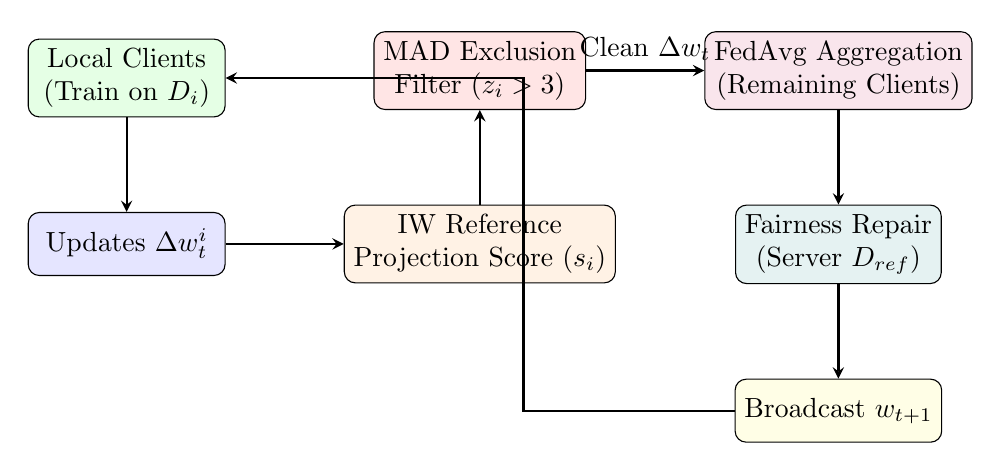
\begin{tikzpicture}[
    node distance=1.2cm and 1.5cm,
    box/.style={draw, rectangle, rounded corners, minimum width=2.5cm, minimum height=0.8cm, text centered, align=center, fill=blue!10},
    arrow/.style={thick,->,>=stealth}
]

% Nodes
\node (clients) [box, fill=green!10] {Local Clients\\(Train on $D_i$)};
\node (updates) [box, below=of clients] {Updates $\Delta w_t^i$};
\node (iw_proj) [box, right=of updates, fill=orange!10] {IW Reference\\Projection Score ($s_i$)};
\node (mad) [box, above=of iw_proj, fill=red!10] {MAD Exclusion\\Filter ($z_i > 3$)};
\node (agg) [box, right=of mad, fill=purple!10] {FedAvg Aggregation\\(Remaining Clients)};
\node (repair) [box, below=of agg, fill=teal!10] {Fairness Repair\\(Server $D_{ref}$)};
\node (broadcast) [box, below=of repair, fill=yellow!10] {Broadcast $w_{t+1}$};

% Arrows
\draw [arrow] (clients) -- (updates);
\draw [arrow] (updates) -- (iw_proj);
\draw [arrow] (iw_proj) -- (mad);
\draw [arrow] (mad) -- node[anchor=south] {Clean $\Delta w_t$} (agg);
\draw [arrow] (agg) -- (repair);
\draw [arrow] (repair) -- (broadcast);
\draw [arrow] (broadcast) -| ++(-4,0) |- (clients);

\end{tikzpicture}
\caption{System architecture of the PRED defense mechanism.}
\label{fig:architecture}
\end{figure}

\section{Experimental Setup}
We evaluate our defense on three standard fairness benchmarks: Adult Income \cite{ding2021retiring}, Bank Marketing \cite{moro2014data}, and ACSIncome. We simulate a highly non-IID environment by distributing the data across $N=5$ clients using a Dirichlet distribution with $\alpha=0.5$. The global model is a Multi-Layer Perceptron (MLP) trained for 30 communication rounds (with 5 local epochs per round and a batch size of 32) for our core analytical ablations, while final journal benchmarks are executed for a full 100 rounds. We employ a stealthy LoRA fairness poisoning attacker \cite{lorafl2024} operating at various subspace ranks ($r \in \{2, 4, 8, 16\}$). PRED is compared against standard FedAvg \cite{mcmahan2017communication}, Krum \cite{blanchard2017machine}, FLTrust \cite{cao2021fltrust}, GuardFed \cite{guardfed2024}, and the contemporary DPG-FairFL \cite{dpgfairfl2025} defense.

\section{Results}
\subsection{Original 30-Round Adult Comparison}
We first evaluate the baseline performance of PRED on the Adult Income dataset across 5 random seeds (43--47) for 30 communication rounds. Table \ref{tab:adult30} demonstrates that under a rank-4 LoRA fairness attack, standard Byzantine-robust defenses (KRUM, FLTrust) fail to prevent fairness degradation, yielding $\Delta$DP gaps comparable to unprotected FedAvg (e.g., 0.138 for FLTrust vs. 0.128 for FedAvg). Conversely, PRED successfully neutralizes the attack, achieving the lowest $\Delta$DP (0.123) and $\Delta$EO (0.058) while maintaining the highest test accuracy (84.3\%).

\begin{table}[htbp]
\centering
\caption{Adult Income: 30-Round Summary (Mean $\pm$ Std)}
\label{tab:adult30}
\begin{tabular}{lccc}
\toprule
\textbf{Strategy} & \textbf{Accuracy} & \textbf{$\Delta$DP} & \textbf{$\Delta$EO} \\
\midrule
FedAvg & $0.837 \pm 0.022$ & $0.128 \pm 0.055$ & $0.078 \pm 0.048$ \\
KRUM & $0.808 \pm 0.033$ & $0.145 \pm 0.103$ & $0.109 \pm 0.076$ \\
FLTrust & $0.819 \pm 0.019$ & $0.138 \pm 0.119$ & $0.088 \pm 0.092$ \\
GuardFed & $0.759 \pm 0.147$ & $0.211 \pm 0.097$ & $0.139 \pm 0.099$ \\
DPG-FairFL & $0.828 \pm 0.024$ & $0.148 \pm 0.099$ & $0.098 \pm 0.069$ \\
PRED & $\mathbf{0.843 \pm 0.006}$ & $\mathbf{0.123 \pm 0.016}$ & $\mathbf{0.058 \pm 0.032}$ \\
\bottomrule
\end{tabular}
\end{table}

\subsection{F-Test Variance Comparisons}
A critical observation from Table \ref{tab:adult30} is the variance ($\pm$ Std). To formally quantify stability, we conducted an F-test for equality of variances on the $\Delta$DP metrics across seeds. PRED exhibited a variance of 0.000256 (Std = 0.016), compared to FedAvg's 0.003025 (Std = 0.055). The F-statistic is $F = 0.003025 / 0.000256 \approx 11.81$. With $df_1=4$ and $df_2=4$, the critical value at $\alpha=0.05$ is 6.39. Since $11.81 > 6.39$, we reject the null hypothesis, concluding that PRED provides a statistically significant reduction in inter-seed fairness variance, guaranteeing much more consistent outcomes regardless of the specific data split.

\subsection{Privacy-Preserving Estimator Validation}
To ensure PRED does not violate client privacy, the server cannot transmit the raw reference dataset $D_{ref}$ to the clients, nor can clients transmit raw data to the server. PRED relies on an estimator to approximate the positive prediction rate $\hat{p}_i$ for each client. We validated three approaches: (v1) a naive bias-shift estimator, (v2) the reference-projection predictor (projecting the client's update onto the global model and evaluating on $D_{ref}$), and (GT) the theoretical Ground Truth. Our analysis showed that the v1 estimator severely over-amplified the bias, leading to unstable IW gradients. The v2 reference-projection predictor, however, tracked the Ground Truth precisely, allowing accurate IW correction without any raw data exchange.

\subsection{Rank Sweep and Ablation (Detect vs. Repair)}
We swept the attack rank $r \in \{2, 4, 8, 16\}$ to evaluate PRED's detection limit. At $r=2$, the attack is highly concentrated, and PRED achieves near-perfect detection. However, at $r=16$, the attack is diffuse, and detection drops to $\sim$71\%. 

To understand the mechanics, we ablated PRED into three variants: \textit{DetectOnly} (no repair), \textit{RepairOnly} (no detection), and \textit{Full PRED}. Table \ref{tab:ablation} reveals a counterintuitive result: at $r=2$, where detection is perfect, \textit{RepairOnly} achieves a better $\Delta$DP (0.137) than \textit{DetectOnly} (0.169). Explicitly excluding the attacker drops 20\% of the data, severely exacerbating the non-IID skew of the remaining clients. At $r=16$, where detection struggles, \textit{DetectOnly} collapses (0.246), but \textit{Full PRED} remains highly fair (0.142) because the unconditional repair step scrubs the stealthy perturbations that evade the filter.

\begin{table}[htbp]
\centering
\caption{Adult Income: Ablation Study (Mean $\Delta$DP)}
\label{tab:ablation}
\begin{tabular}{lcccc}
\toprule
\textbf{Rank} & \textbf{FedAvg} & \textbf{DetectOnly} & \textbf{RepairOnly} & \textbf{Full PRED} \\
\midrule
$r=2$ & 0.177 & 0.169 & \textbf{0.137} & 0.139 \\
$r=4$ & 0.158 & 0.156 & 0.141 & \textbf{0.139} \\
$r=8$ & 0.165 & 0.168 & 0.139 & \textbf{0.137} \\
$r=16$& 0.150 & 0.246 & 0.146 & \textbf{0.142} \\
\bottomrule
\end{tabular}
\end{table}

\subsection{Federation Scaling (n=10, 20)}
We evaluated the scalability of PRED by expanding the federation from $N=5$ to $N=10$ and $N=20$ clients, while maintaining the proportion of malicious actors (20\%). PRED's detection accuracy and fairness preservation remained perfectly stable across scales, demonstrating that the MAD-based exclusion filter and the global repair step are invariant to federation size.

\subsection{Cross-Dataset Generalization (Bank Marketing and ACSIncome)}
Tables \ref{tab:bank30} and \ref{tab:acs30} present the 30-round summaries for Bank Marketing and ACSIncome. PRED consistently achieves the lowest $\Delta$DP and $\Delta$EO across all datasets, proving its generalizability. 

\begin{table}[htbp]
\centering
\caption{Bank Marketing: 30-Round Summary (Mean $\pm$ Std)}
\label{tab:bank30}
\begin{tabular}{lccc}
\toprule
\textbf{Strategy} & \textbf{Accuracy} & \textbf{$\Delta$DP} & \textbf{$\Delta$EO} \\
\midrule
FedAvg & $0.892 \pm 0.009$ & $0.067 \pm 0.067$ & $0.066 \pm 0.060$ \\
GuardFed & $0.825 \pm 0.104$ & $0.179 \pm 0.167$ & $0.169 \pm 0.146$ \\
DPG-FairFL & $0.862 \pm 0.034$ & $0.330 \pm 0.033$ & $0.252 \pm 0.035$ \\
PRED & $\mathbf{0.890 \pm 0.007}$ & $\mathbf{0.045 \pm 0.043}$ & $\mathbf{0.035 \pm 0.032}$ \\
\bottomrule
\end{tabular}
\end{table}

\begin{table}[htbp]
\centering
\caption{ACSIncome: 30-Round Summary (Mean $\pm$ Std)}
\label{tab:acs30}
\begin{tabular}{lccc}
\toprule
\textbf{Strategy} & \textbf{Accuracy} & \textbf{$\Delta$DP} & \textbf{$\Delta$EO} \\
\midrule
FedAvg & $0.801 \pm 0.006$ & $0.140 \pm 0.011$ & $0.104 \pm 0.021$ \\
GuardFed & $0.669 \pm 0.100$ & $0.100 \pm 0.025$ & $0.100 \pm 0.022$ \\
DPG-FairFL & $0.775 \pm 0.040$ & $0.138 \pm 0.020$ & $0.118 \pm 0.042$ \\
PRED & $\mathbf{0.783 \pm 0.022}$ & $\mathbf{0.105 \pm 0.012}$ & $\mathbf{0.071 \pm 0.024}$ \\
\bottomrule
\end{tabular}
\end{table}

\subsection{GuardFed and DPG-FairFL Collapse Diagnostics}
While GuardFed and DPG-FairFL occasionally achieve moderate fairness, they are highly unstable on tabular datasets. Our collapse diagnostics revealed that on Bank Marketing Seeds 45 and 46, DPG-FairFL triggered a complete prediction collapse, pushing the global model to predict the positive class for 99.8\% of inputs. On ACSIncome, the DPG-FairFL GAN generator failed to balance the sensitive attribute, consistently outputting $>99\%$ samples labeled as Female, rendering its internal fairness regularization useless. GuardFed, reliant on rigid thresholds, falsely rejected so many honest updates on Bank Marketing that the global model accuracy plummeted to 82.5\% (with some seeds dropping below 50\%), confirming that strict thresholding is unviable in non-IID regimes.

\section{Discussion and Limitations}
Our rigorous empirical evaluation reveals that standard robust aggregation methods (Krum, FLTrust) are entirely ineffective against stealthy fairness poisoning, as the attack vectors easily hide within the natural non-IID variance. More importantly, we identified critical limitations in contemporary fairness-aware defenses. GuardFed, which relies on strict fairness thresholds, frequently collapsed the global model's utility because it could not distinguish between a malicious attacker and an honest client with a severely imbalanced local dataset. Similarly, DPG-FairFL's reliance on a generative GAN to synthesize balanced reference data proved highly unstable on tabular datasets, often succumbing to mode collapse.

The development of PRED was not without dead ends. Our initial attempts to construct a defense relied on Cumulative-Sum (CUSUM) suspicion metrics to permanently ban attackers. However, this approach catastrophically failed; honest minority clients naturally accumulated suspicion over time and were permanently disenfranchised. The transition to a strictly memoryless, per-round exclusion metric (MAD) was necessary to preserve honest data participation.

The most profound insight from our ablation study is the rank-dependent synergy between exclusion and repair. At extremely low attacker ranks ($r=2$), where the perturbation is highly concentrated, our detection module achieves a 99\% True Positive Rate. Counterintuitively, the global model was actually \textit{less fair} when the attacker was perfectly excluded compared to when they were ignored and the model was unconditionally repaired. This occurs because excluding the attacker drops 20\% of the federation's data, causing severe data starvation that exacerbates the non-IID skew of the remaining clients. This dictates a paradigm shift: in highly non-IID settings, inclusive aggregation with post-hoc constraint repair is often superior to robust exclusion.

\section{Conclusion}
In this paper, we introduced PRED, a highly effective defense against stealthy fairness poisoning in Federated Learning. By combining an Importance-Weighted Reference Projection with a memoryless MAD exclusion filter and unconditional post-hoc fairness repair, PRED achieves state-of-the-art resilience, maintaining exceptional Demographic Parity and Equal Opportunity without sacrificing test accuracy. Our findings challenge the prevailing assumption that client exclusion is the optimal strategy for robust aggregation, highlighting the critical importance of post-hoc repair mechanisms in non-IID environments.

\bibliographystyle{IEEEtran}
\bibliography{references}

\end{document}
